\documentclass[17pt,xcolor=table]{beamer} 
\setbeamersize{text margin left=0cm,text margin right=0.25cm}
\mathversion{bold}
%\usepackage{paralist}
\usepackage{beamerthemesplit}
\usepackage{beamerthemeshadow}
\definecolor{Green}{RGB}{0,190,0}
\definecolor{Brown}{RGB}{205,0,0}
\setbeamercolor{structure}{fg=Brown}
\setbeamercolor{alerted text}{fg=Brown}
\logo{
\includegraphics[height=0.7cm]{FOSSEE.jpeg}\hspace{9.7cm}

\includegraphics[height=1cm]{ST-logo.jpeg}}
\hyphenation{phosphorylated}

\begin{document}
\sffamily \bfseries
\title
[Lighting an LED on Shield from Arduino IDE]
{Lighting an LED on Shield \\ from the Arduino IDE}
\author [Manas,Rupak,Kannan]
{\small Spoken Tutorial Project \\
http://spoken-tutorial.org \\ [0.3cm]
  National Mission
  on Education 
  through ICT \\ 
  http://sakshat.ac.in \\ [0.3cm]
  Manas, Rupak, Kannan \\ IIT Bombay \\ [0.35cm]
\small 3 July 2015}
\date{}
\begin{frame}
   \titlepage
\end{frame}

\begin{frame}
\frametitle{Learning Objectives}
\vspace{-0.25in}
We will learn to 
\begin{itemize}
\item Connect an Arduino Uno board to a computer
\item Identify the port number
\item Load the firmware on to the Arduino Uno board
\item Turn the LED on using Arduino IDE
\end{itemize}
\end{frame}

\begin{frame}
\frametitle{System Requirements}
\begin{itemize}
\item Windows 8, 64bit
\item Arduino IDE 1.6.5
\item Arduino Uno board
\item Shield
\end{itemize}
\end{frame}

\begin{frame}
\frametitle{Connecting Shield to Uno}
\centerline{
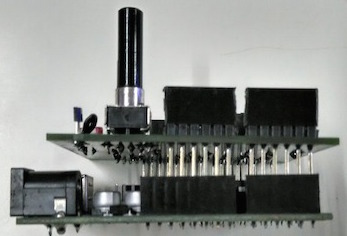
\includegraphics[width=0.9\linewidth]{figures/shield-crop.jpg}
}
\end{frame}

\begin{frame}
\frametitle{Two ends of USB cable}
\centerline{
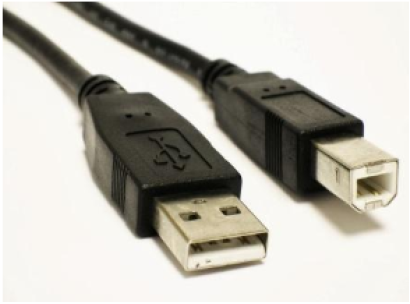
\includegraphics[width=0.9\linewidth]{figures/cable.png}
}
\end{frame}

\begin{frame}
\frametitle{Connecting USB cable with Uno}
\centerline{
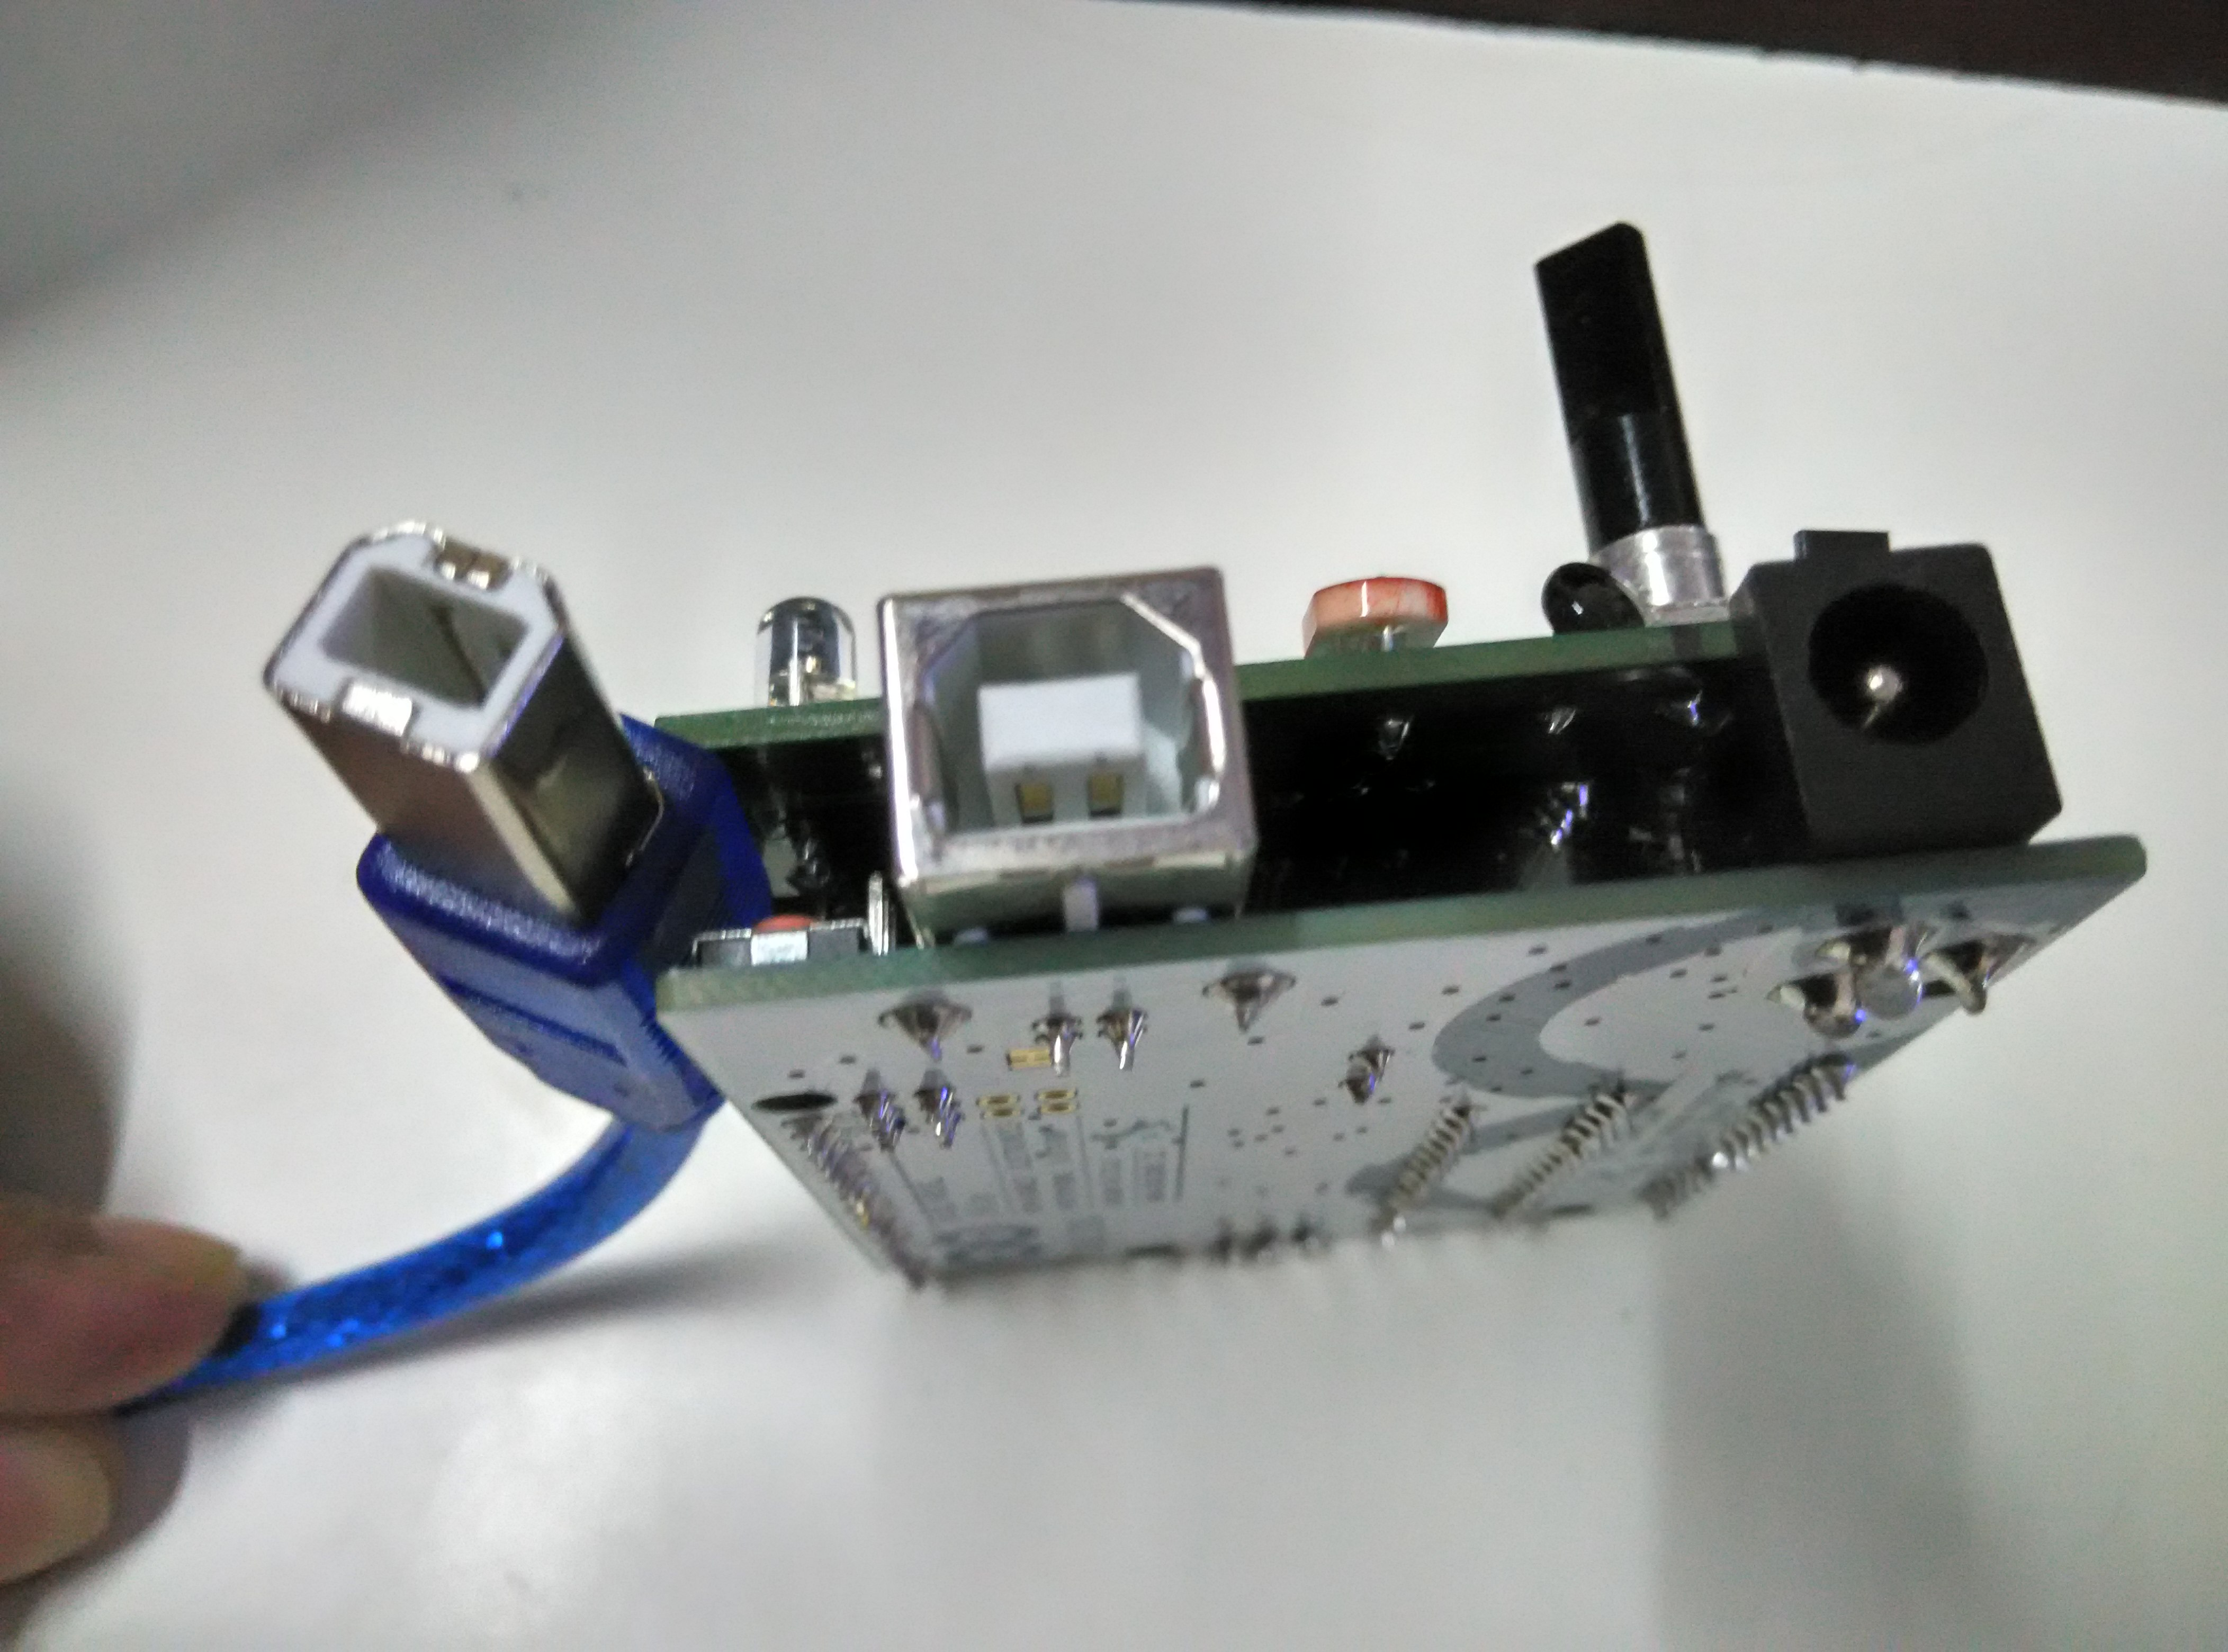
\includegraphics[width=0.9\linewidth]{figures/USB.jpg}
}
\end{frame}

\begin{frame}
\frametitle{Shield's Blue LED is on}
\centerline{
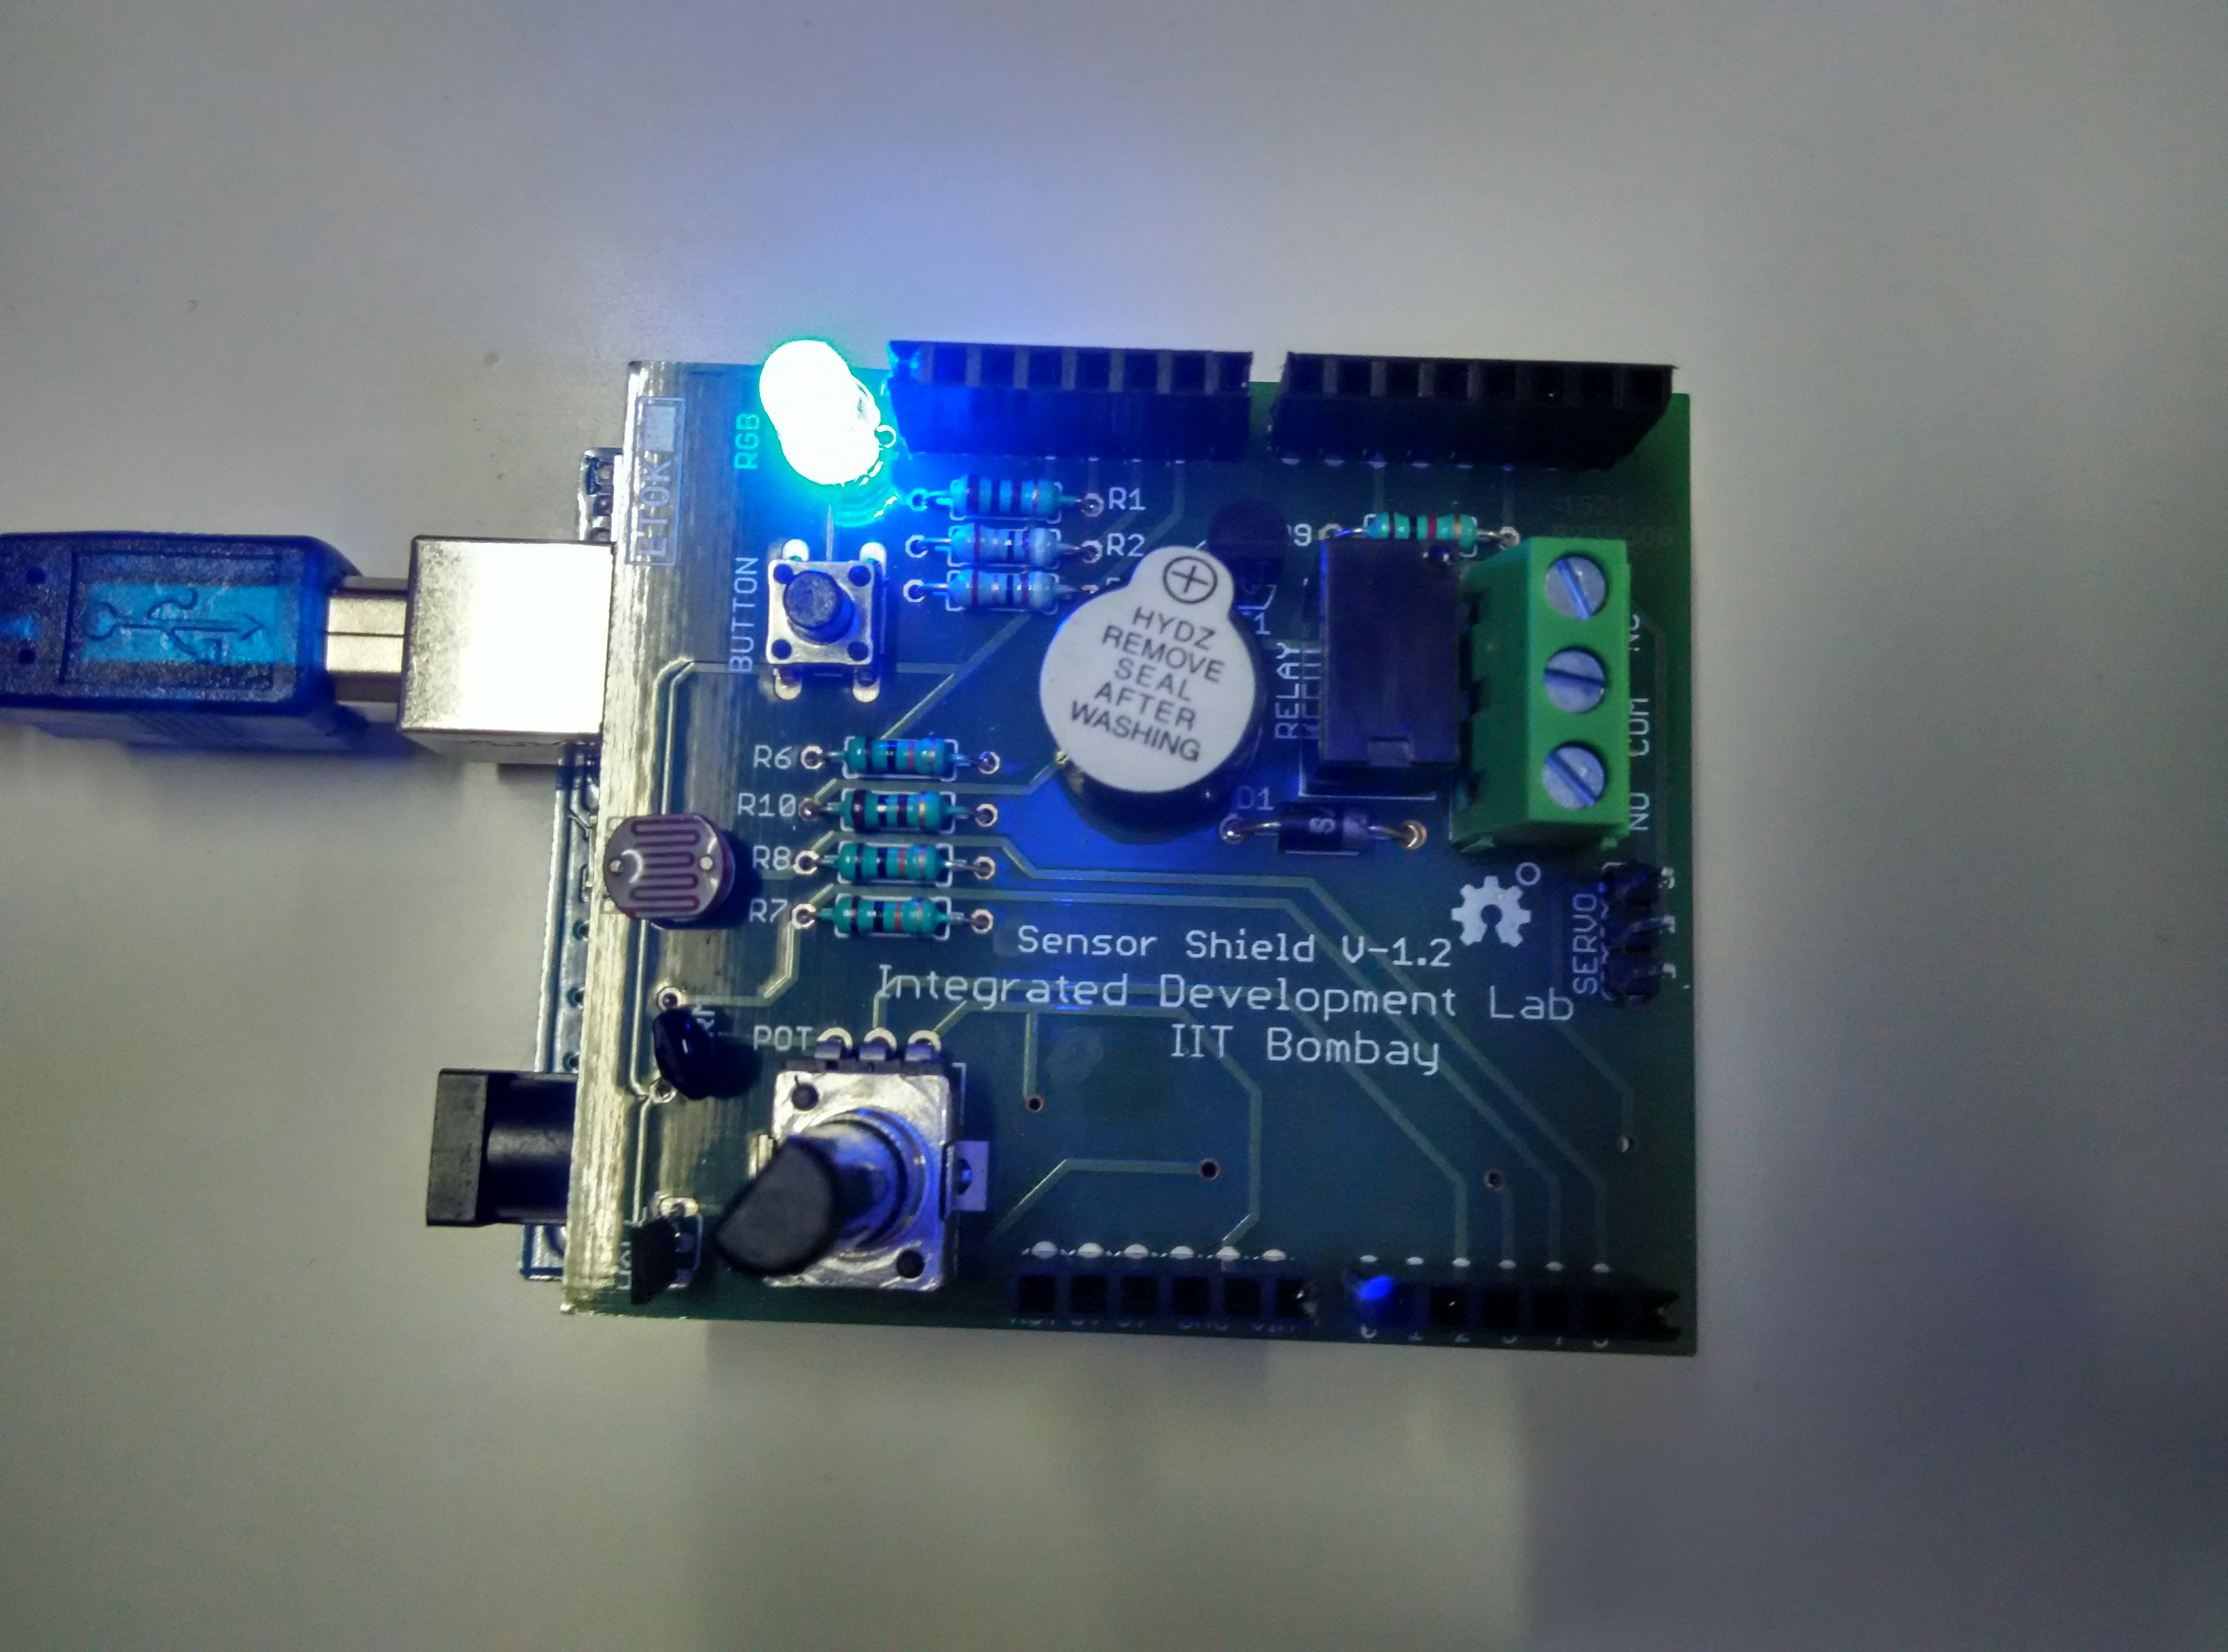
\includegraphics[width=0.9\linewidth]{figures/LED.jpg}
}
\end{frame}

\begin{frame}
  \frametitle{Summary}
  \begin{itemize}
  \item Connected an Arduino Uno board to a computer
  \item Identified the port number
  \item Loaded the firmware on to the Arduino Uno board
  \item Turned on the blue LED on the shield
  \end{itemize}
\end{frame}

\begin{frame}
  \frametitle{Assignment 1}
  \begin{itemize}
  \item Turn the green led on by putting 1 on pin 10
  \item Turn the red led on by putting 1 on pin 11
  \end{itemize}
\end{frame}

\begin{frame}
  \frametitle{Assignment 2: From book}
  \begin{itemize}
  \item We have a written a Scilab-Arduino control book
  \item It is published by Shroff Publishers, Mumbai
  \item An e-copy is available for free download from fossee.in
  \item Carry out the other LED lighting experiments explained in the
    book
  \end{itemize}
\end{frame}

\begin{frame}
\frametitle{About the Spoken Tutorial Project}
\begin{itemize}
\item Watch the video available at {\color{blue} http://spoken-tutorial.org /What\_is\_a\_Spoken\_Tutorial}
\item It summarises the Spoken Tutorial project \pause
\item If you do not have good bandwidth, you can download and watch it
\end{itemize}
\end{frame}

\begin{frame}
\frametitle{Spoken Tutorial Workshops}
The Spoken Tutorial Project Team
\begin{itemize}
\item Conducts workshops using spoken tutorials
\item Gives certificates to those who pass an online test
\item For more details, please write to {\color{blue} contact@spoken-tutorial.org}
\end{itemize}
\end{frame}

\begin{frame}
\frametitle{Forum to answer questions}
\vspace{-0.5in}
\begin{itemize}
\item Do you have questions in THIS Spoken Tutorial?
\item Choose the minute and second where you have the question.
\item Explain your question briefly.
\item Someone from the FOSSEE team will answer them.
\end{itemize}
Please visit {\small \color{blue}
  http://forums.spoken-tutorial.org/} 
\end{frame}

\begin{frame}
\frametitle{Textbook Companion Project}
\begin{itemize}
\item The FOSSEE team coordinates coding of solved examples of popular
  books 
\item We give honorarium and certificate to those who do this
\end{itemize}
For more details, please visit this site: 
{\color{blue} http://fossee.in}
\end{frame}

\begin{frame}
\frametitle{Lab Migration Project}
\begin{itemize}
\item The FOSSEE team helps migrate commercial simulator labs to DWSIM
\item We give honorarium and certificates to those who do this
\end{itemize}
For more details, please visit this site: 
{\color{blue} http://fossee.in}
\end{frame}

\begin{frame}
\frametitle{Acknowledgements}
\begin{itemize}
\item Spoken Tutorial and FOSSEE are funded by the National Mission on
  Education through ICT, MHRD, Government of India
\item More information on this mission is available at \\
\hspace{0.25in}
{\small \color{blue}http://spoken-tutorial.org/NMEICT-Intro}
\end{itemize}
\end{frame}

\begin{frame}
\frametitle{Thanks!}
\end{frame}

\end{document}

